\section{Estudio de Factibilidad}

\newcommand{\tabitem}{~~\llap{\textbullet}~~}

El estudio de factibilidad sirve para estimar los recursos necesarios para el desarrollo del proyecto, el éxito de la implementación está determinado por el grado de factibilidad que se presente en tres aspectos a evaluar: técnico, económico y operativo.

\subsection{Factibilidad Técnica}

La factibilidad técnica consiste en realizar una evaluación de la tecnología con la que cuenta el equipo de trabajo, en éste estudio se muestra la información recolectada sobre los componentes técnicos con los que se cuenta y la posibilidad de hacer uso de los mismos en el desarrollo e implementación del sistema propuesto y de ser necesario, los requisitos tecnológicos que deben ser adquiridos para el desarrollo y puesta en marcha del sistema. 

De acuerdo a los requisitos del sistema se evaluaron sus componentes bajo dos enfoques: hardware y software. 

\subsubsection{Hardware}

Respecto al hardware, se requieren equipos de cómputo para: desarrollar la aplicación móvil, alojar la aplicación Web de administración y tener el servicio Web funcionando. También es necesario un telefono inteligente que cuente con los sensores necesarios para la localización en interiores. 

El equipo de trabajo cuenta con las computadoras personales para el desarrollo de la aplicación móvil, las cuales se detallan en la Tabla \ref{tab:hardware}.

\begin{table}[h] 
	\begin{center}
		\begin{tabular}{|c|c|}
			\hline \rowcolor[RGB]{0,102,204} 
			\textcolor{blanco}{\bf Recurso} &
				\textcolor{blanco}{\bf Características} \\
			\hline \rowcolor[RGB]{224,224,224} 
			\multirow{1}{2.8cm}{Laptop Lenovo} &
				{\parbox{0.5\textwidth}{
					\begin{itemize}
                			\item Procesador Intel Core i3 2.2 GHz
		               	\item 4 GB memoria RAM DDR3
                			\item 520 GB de disco duro
                			\item Sistema Operativo Windows 7 de 64 bits
           			\end{itemize} }} \\
      		\hline 
      		\multirow{1}{2.8cm}{MacBook Pro} &
      				{\parbox{0.5\textwidth}{
					\begin{itemize}
                			\item Procesador Intel Core i7 2.3 GHz
		               	\item 8 GB memoria RAM
                			\item 250 GB de almacenamiento en flash
                			\item Sistema Operativo OS X 10.10.1
           			\end{itemize} }} \\
      		\hline 
		\end{tabular}
	\end{center}
	\caption[Recursos de Hardware del Equipo]{Recursos de Hardware del Equipo} 
	\label{tab:hardware}
\end{table}

Debido a la naturaleza del sistema a desarrollar, se requiere de ciertos dispositivos móviles con las características necesarias para poder implementar y elaborar las pruebas necesarias a la aplicación móvil. En la Tabla \ref{tab:reqMin} se enlistan las características mínimas requeridas en dichos dispositivos móviles para el correcto funcionamiento de la aplicación.

\begin{table}[h] 
	\begin{center}
		\begin{tabular}{|>{\columncolor[RGB]{0,102,204}}l|l|}
			\hline  
			\textcolor{blanco}{\bf Sistema Operativo} &
				{\parbox{0.5\textwidth}{
					\begin{itemize}
                			\item iOS 7 o superior
		               	\item Android 4.3 o superior
           			\end{itemize} }} \\
			\hline 
			\textcolor{blanco}{\bf Procesador} &
				\hspace{0.5cm}1.3 GHz \\
      		\hline 
      		\textcolor{blanco}{\bf Memoria RAM} &
				\hspace{0.5cm}1 GB \\
      		\hline 
      		\textcolor{blanco}{\bf Sensores} &
				{\parbox{0.5\textwidth}{
					\begin{itemize}
                			\item Magnetómetro (Brújula)
		               	\item Acelerómetro
		               	\item Giroscopio
           			\end{itemize} }} \\
			\hline 
		\end{tabular}
	\end{center}
	\caption[Requerimientos mínimos del dispositivo móvil]{Requerimientos mínimos del dispositivo móvil} 
	\label{tab:reqMin}
\end{table}

Se cuenta con dos dispositivos que cumplen con los requerimientos mínimos, uno con el sistema operativo Android y otro con iOS. Debido a ciertas ventajas (descritas en la sección \ref{SOM}) que se tienen al momento del desarrollo, se utilizará el dispositivo móvil con sistema operativo Android. Este dispositivo será utilizado para realizar las actividades correspondientes durante las etapas de producción, estabilización y pruebas. En la tabla \ref{tab:movilesPos} se describen algunas especificaciones técnicas del dispositivo.

\begin{table}[h] 
	\begin{center}
		\begin{tabular}{|>{\columncolor[RGB]{0,102,204}}l|l|}
			\hline  
			\textcolor{blanco}{\bf Modelo} &
				\hspace{0.5cm}Samsung Galaxy S4\\
			\hline
			\textcolor{blanco}{\bf Sistema Operativo} &
				\hspace{0.5cm}Android 4.4.2 KitKat \\
      		\hline 
      		\textcolor{blanco}{\bf Pantalla} &
				\hspace{0.5cm}5 pulgadas \\
      		\hline
      		\textcolor{blanco}{\bf Resolución de Pantalla} &
				\hspace{0.5cm}1,920 x 1,080 pixeles (441 ppp) \\
      		\hline 
      		\textcolor{blanco}{\bf Procesador} &
				\hspace{0.5cm}Qualcomm Snapdragon 600 1.9 GHz \\
      		\hline 
			\textcolor{blanco}{\bf Memoria RAM} &
				\hspace{0.5cm}2 GB \\
      		\hline 
      		\textcolor{blanco}{\bf Conectividad} &
				\hspace{0.5cm}3G \\
      		\hline 
      		\textcolor{blanco}{\bf Sensores} &
				{\parbox{0.5\textwidth}{
					\begin{itemize}
                			\item Magnetómetro (Brújula)
		               	\item Acelerómetro
		               	\item Giroscopio
           			\end{itemize} }} \\
			\hline 
		\end{tabular}
	\end{center}
	\caption[Específicaciones técnicas Galaxy S4]{Específicaciones técnicas Galaxy S4} 
	\label{tab:movilesPos}
\end{table}

\subsubsection{Software}

El software que se necesita consta de sistemas operativos, tanto de escritorio como móvil; entorno de desarrollo integrado (IDE, sigla en ingles de Integrated Development Environment), una herramienta UML, un sistema gestor de base de datos (SGBD) y se utilizarán algunas APIs.

\paragraph{Sistema Operativo Móvil}

\label{SOM}

En la Tabla \ref{tab:comSOM} se muestran los diferentes sistemas operativos móviles que nos sirven para desarrollar la aplicación móvil.

\begin{table}[h] 
	\begin{center}
		\begin{tabular}{|>{\columncolor[RGB]{0,102,204}}p{4cm}|>{\columncolor[RGB]{102,204,0}}p{4.5cm}|p{4.5cm}|}
			\hline  
			\textcolor{blanco}{\bf Sistema Operativo} &
				\hspace{0.5cm}Android &
				\hspace{0.5cm}iOS \\
			\hline
			\textcolor{blanco}{\bf Desarrollador} &
				\hspace{0.5cm}Google &
				\hspace{0.5cm}Apple Inc. \\
      		\hline 
      		\textcolor{blanco}{\bf Imagen \newline Representativa} &
				{\raisebox{-\totalheight}{\hspace{0.5cm}
\includegraphics[width=15mm, height=15mm]{Figuras/android.png}}} &
				{\raisebox{-\totalheight}{\hspace{0.5cm}
\includegraphics[width=15mm, height=15mm]{Figuras/ios.png}}} \\
      		\hline
      		\textcolor{blanco}{\bf Plataforma de \newline Desarrollo} &
				\hspace{0.5cm}Windows, Mac OS y Linux. &
				\hspace{0.5cm}Mac OS \\
      		\hline 
      		\textcolor{blanco}{\bf Variedad de \newline Dispositivos} &
				\hspace{0.5cm}Muy Alta &
				\hspace{0.5cm}Baja \\
      		\hline 
			\textcolor{blanco}{\bf Número de \newline Aplicaciones \newline Disponibles} &
				\hspace{0.5cm}1.3 millones &
				\hspace{0.5cm}1.2 millones \\
      		\hline  
      		\textcolor{blanco}{\bf Arquitectura} &
				{\parbox{0.5\textwidth}{
					\begin{itemize}
                			\item Kernel de Linux
		               	\item Librerías
		               	\item Android Runtime
		               	\item Framework de Apps
           			\end{itemize} }} &
				{\parbox{0.5\textwidth}{
					\begin{itemize}
                			\item Core OS
		               	\item Core Services
		               	\item Media
		               	\item Cocoa Touch
           			\end{itemize} }} \\
			\hline 
			\textcolor{blanco}{\bf Tipo de Código de Desarrollo} &
				\hspace{0.5cm}Abierto &
				\hspace{0.5cm}Cerrado \\
      		\hline  
      		\textcolor{blanco}{\bf Costo de Licencia \newline para Desarrollo} &
				\hspace{0.5cm}\$ 25.00 USD. Pago Único  &
				\hspace{0.5cm}\$ 99.00 USD. Pago Anual \\
      		\hline  
      		\textcolor{blanco}{\bf Proceso de validación de aplicaciones} &
				\hspace{0.5cm}Bastante flexible de 5 a 30  minutos &
				\hspace{0.5cm}Muy estricto de 1 \newline semana en  promedio \\
      		\hline  
      		\textcolor{blanco}{\bf IDE (Entorno de Desarrollo Integrado)} &
				\hspace{0.5cm}ADT y Android Studio &
				\hspace{0.5cm}Xcode \\
      		\hline  
      		\textcolor{blanco}{\bf Lenguajes de \newline Programación} &
				\hspace{0.5cm}C, C++ y Java. &
				\hspace{0.5cm}Objective-C, C, C++ y Swift. \\
      		\hline  
      		\textcolor{blanco}{\bf Uso en el mercado} &
				\hspace{0.5cm}78.4 \% del mercado&
				\hspace{0.5cm}15.6 \% del mercado \\
      		\hline  
		\end{tabular}
	\end{center}
	\caption[Comparación de Sistemas Operativos Móviles]{Comparación de Sistemas Operativos Móviles} 
	\label{tab:comSOM}
\end{table}

Como podemos observar en la Tabla \ref{tab:comSOM}, con Android tenemos más opciones en la plataforma de desarrollo, lo cual se adecua de buena forma con los equipos que contamos. La presencia en el mercado y el costo de licencia para desarrollo, hacen que nos decidamos por Android como sistema operativo móvil para desarrollar TASMC.

\subparagraph{Android}

Android permite programar en un entorno de trabajo (framework) de Java, aplicaciones sobre una maquina virtual Dalvik (una variación de la máquina virtual de Java con compilación en tiempo de ejecución). Además, a diferencia de otros sistemas operativos, Android es de código libre lo que permite mayores ventajas para el desarrollo de nuevas aplicaciones, o incluso, modificar el propio sistema operativo. Aunado a esto, en los últimos años Android se ha posicionado como el líder mundial dentro de las plataformas para dispositivos móviles disponibles en el mercado. \cite{Android}

\subparagraph{Versiones de Android}

Una vez que se ha justificado la elección de Android como el sistema operativo al cual estará orientado nuestro sistema, debemos establecer que versión de dicho sistema operativo es la indicada para que la aplicación móvil se desempeñe satisfactoriamente. De acuerdo a los datos ofrecidos en la página oficial de Android, la versión con mayor presencia en el mercado hasta el mes de Agosto de 2014 es la 4.3 Jelly Bean pero no cumple con los requerimientos que necesita el sistema para funcionar por lo que se opto por el segundo de mayor presencia y la cual es la versión más reciente 4.4 KitKat, dicha versión ofrece las funcionalidades y compatibilidad requeridas por nuestro sistema. En la Figura \ref{fig:versionesFigura} y la Tabla \ref{tab:versionesTabla} se muestran las estadísticas referentes a la presencia en el mercado de cada una de las versiones de Android.

\begin{figure}[htbp]
	\centering
		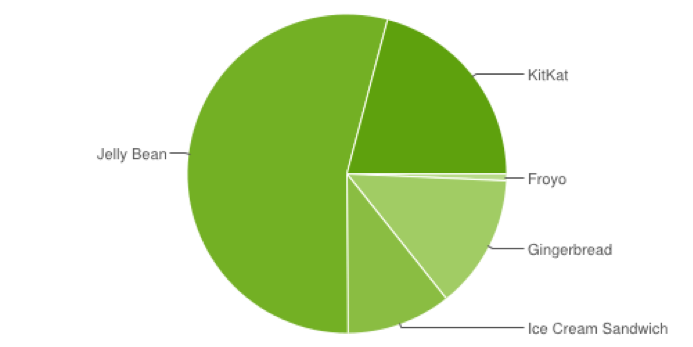
\includegraphics[width=1\textwidth]{Figuras/versionesAndroid.png}
		\rule{30em}{0.5pt}
	\caption[Gráfica de Usabilidad de las Versiones de Android]{Gráfica de Usabilidad de las Versiones de Android (Agosto 2014) \cite{devAndroid}}
	\label{fig:versionesFigura}
\end{figure}

\begin{table}[h] 
	\begin{center}
		\begin{tabular}{|c|c|c|c|}
			\hline \rowcolor[RGB]{0,102,204} 
			\textcolor{blanco}{\bf Versión} &
				\textcolor{blanco}{\bf Nombre} &
				\textcolor{blanco}{\bf API} &
				\textcolor{blanco}{\bf Presencia en el Mercado} \\
			\hline \rowcolor[RGB]{224,224,224} 
				2.2 &
				Froyo &
				8 &
				0.7\% \\
      		\hline 
      			2.3.3 - 2.3.7 &
				Gingerbread &
				10 &
				13.6\% \\
      		\hline \rowcolor[RGB]{224,224,224} 
      			4.0.3 - 4.0.4 &
				Ice Cream Sandwich &
				15 &
				10.6\% \\
      		\hline 
      			4.1.x &
				Jelly Bean &
				16 &
				26.5\% \\
      		\hline \rowcolor[RGB]{224,224,224} 
      			4.2.x &
				Jelly Bean &
				17 &
				19.8\% \\
      		\hline 
      			4.3 &
				Jelly Bean &
				18 &
				7.9\% \\
      		\hline \rowcolor[RGB]{224,224,224} 
      			4.4 &
				KitKat &
				19 &
				20.9\% \\
      		\hline 
		\end{tabular}
	\end{center}
	\caption[Usabilidad de las Versiones de Android]{Usabilidad de las Versiones de Android \cite{devAndroid}} 
	\label{tab:versionesTabla}
\end{table}

\paragraph{Lenguaje de Programación}

La fila correspondiente a lenguajes de programación en la Tabla \ref{tab:comSOM} nos muestra C, C++ y Java como los mas utilizados para Android. En la Tabla \ref{tab:paramLengu} se muestran los parámetros de los lenguajes de programación que aparecen en la Tabla \ref{tab:lenguProgra}, esto con el fin de elegir el lenguaje de programación que se utilizará en este proyecto. 


